\section{Control Dinámico del brazo}
En esta última parte del proyecto, una vez se conoce el modelo del robot en las diferentes configuraciones, se pasará a buscar implementar un control dinámico sobre el mismo.Para poder implementar controladores sobre nuestro robot, será necesario obtener una función de transferencia matemática a modo de modelo que se asemeje al robot real.\\
Una vez se tenga un modelo lineal de cada articulación del robot, junto con el generador de trayectorias creado anteriormente, se buscará que el robot siga una trayectoria predefinida.\\

	\subsection{Obtención del modelo lineal de las articulaciones del brazo}
Para obtener la función de transferencia de cada articulación del robot, se linealizará la ecuación dinamica que define cada motor en un punto de equilibrio en torno a velocidades nulas. Por lo tanto, las consideraciones que se tendrán en cuenta para linealizar la ecuación dinamica que define el comportamiento de cada articulacion del robot son:
\begin{itemize}
	\item Velocidades de equilibrio
	\begin{center}
		$ \dot{q_{eq}}=0 rad/s $\\
		$ \dot{q} =\dot{q_{eq}}+\Delta\dot{q}$
	\end{center}
	\item Aceleraciones de equilibrio
\begin{center}
	$ \ddot{q_{eq}}=0 rad/s $\\
	$  $
	$ \ddot{q} =\ddot{q_{eq}}+\Delta\ddot{q}$
\end{center}
\end{itemize}

Ademas de ello, se aplicarán una serie de simplificaciones a la ecuación dinámica. A continuación, se mostrarán las ecuaciones dinámicas de los motores:\\
\begin{center}
	$$
	\begin{pmatrix}
	 \tau_{1} \\
	 \tau_{2} \\
	 \tau_ {3}
	\end{pmatrix}=
	\begin{pmatrix}
	Kt_{1}R_{1}Im_{1}  \\
	Kt_{2}R_{2}Im_{2}  \\
	Kt_{3}R_{3}Im_{3}
	\end{pmatrix} =
	\begin{pmatrix}
	Ma_{11} & Ma_{12} & Ma_{13}  \\
	Ma_{21} & Ma_{22} & Ma_{23}  \\
	Ma_{31} & Ma_{32} & Ma_{33}
	\end{pmatrix}
	\ddot{q}+
	\begin{pmatrix}
	Va_{1} \\
	Va_{2} \\
	Va_{3} \\
	\end{pmatrix}
	\dot{q}+
	\begin{pmatrix}
	Ga_{1}  \\
	Ga_{2}  \\
	Ga_{3}\\
	\end{pmatrix}
	$$
\end{center}
donde se asume que dentro de los términos de inercia y de Coirolis se han tenido en cuenta las inercias y fricciones viscosas de los motores.\\

La primera simplificación del modelo que se hará para poder linealizar el modelo en torno a un punto de operación, será suponer la matriz de inercias diagonal y, además de ello, se cogerá el valor medio de todos los senos y cosenos de tal modo que únicamente se tomen los valores de inercias medios. De éste modo, se desacoplará el sistema.\\
En cuando a la matriz de términos de Coirolis, únicamente aportarán a la linealización la fricción viscosa de los motores. Por último, la gravedad se despreciará para obtener un modelo, de tal modo que, se emplearán las siguientes ecuaciones para obtener los modelos de las articulaciones del robot:
\begin{equation}
	\begin{pmatrix}
	Kt_{1}R_{1}Im_{1}  \\
	Kt_{2}R_{2}Im_{2}  \\
	Kt_{3}R_{3}Im_{3}
	\end{pmatrix} =
	\begin{pmatrix}
	Ma_{11} & 0 	  & 0  \\
		0   & Ma_{22} & 0  \\
		0   & 0   	  & Ma_{33}
	\end{pmatrix}
	\ddot{q}+
	\begin{pmatrix}
	Va_{1} \\
	Va_{2} \\
	Va_{3} \\
	\end{pmatrix}
	\dot{q}
\end{equation}

A continuación, se obtendrá el modelo de la primera articulación y, el procedimiento será análogo para las restantes:
\begin{center}
	$Kt_{1}R_{1}Im_{1}(t)=Ma_{11}\ddot{q_{1}(t)} + Va_{1}\dot{q_{1}(t)}$
\end{center}
Se realizará una transformación al dominio de Laplace y, posteriormente, se expresará en forma de función de transferencia:
\begin{center}
	$Kt_{1}R_{1}Im_{1}(s)=s^{2}Ma_{11}q_{1}(s) + sVa_{1}q_{1}(s)$ $\rightarrow$ $\frac{q_{1}(s)}{Im_{1}(s)}=\frac{Kt_{1}R_{1}}{s(Ma_{11}s+Va_{1})}$
\end{center}

Por lo tanto, se definirá el modelo de cada articulación cómo:
\begin{equation}
	G_{1}(s)=\frac{Kt_{1}R_{1}}{s(Ma_{11}s+Va_{1})} \hspace{1cm} G_{2}(s)=\frac{Kt_{2}R_{2}}{s(Ma_{2}s+Va_{2})} \hspace{1cm} G_{3}(s)=\frac{Kt_{3}R_{3}}{s(Ma_{33}s+Va_{3})}
\end{equation}
\newpage
	\subsection{Diseño de controladores}
	En éste apartado, se analizará cómo se hayarán los controladores que, posteriormente se implementarán sobre el robot para hacer que se traslade a lo largo de una trayectoria que se generará mediante el control cinemático.\\
	Cabe destacar que, en los controladores que se implementen junto con el compensador de gravedad, el de dinámica o el par calculado, la realimentación podría ser por referencia, en lugar de emplear las medidas reales, de tal modo que se realimente con una señal sin ruido ni errores.

	\subsubsection{Controlador PD/PID}
	\subsubsection{Controlador PD/PID con compensación de gravedad}
	Para implementar éste controlador, se parte de la base de que, aunque la gravedad es una perturbación mantenida, se puede
modelar, ya que se conoce de la obtención del modelo dinámico los efectos de la gravedad en el modelo del robot.\\
Por tanto, para implementar un controlador con compensación de gravedad se le sumará a la señal de control generada por el
controlador los efectos de la gravedad en el robot.\\
Este bloque que añade los efectos de la gravedad tendrá como entrada la posición actual del robot y la salida será la compensación de la señal de control. El esquema de montaje de éste tipo de control se muestra a continuación:

\begin{figure}[h!]
	\centering
	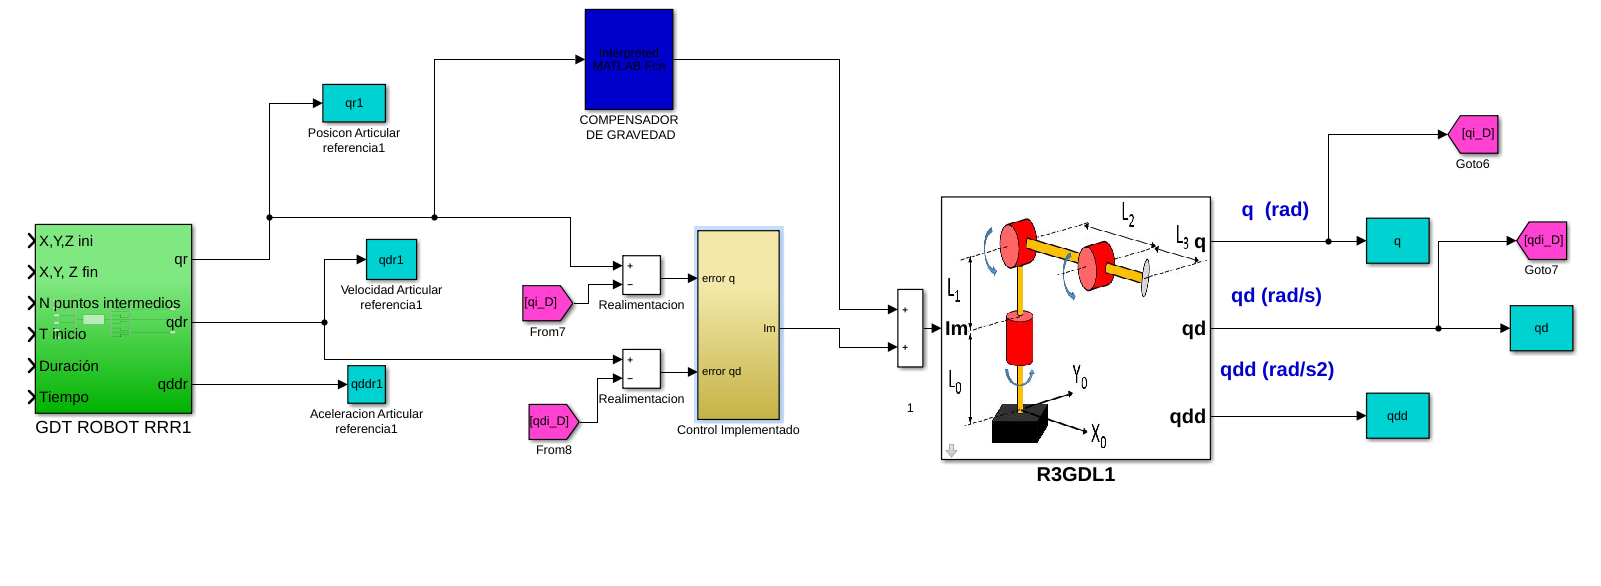
\includegraphics[width=.8\textwidth]{montaje_grav}
	\caption{Diagrama de control del compensador de gravedad}
\end{figure}

	\subsubsection{Controlador PD/PID con compensación de dinámica (Feedforward)}
	Para implementar éste controlador, también conocido como \textit{Feedforward}, se modificará el modelo de control de tal modo que se precompensen los efectos del modelo dinámico completo del robot, no solo la gravedad.
	\begin{equation}
		I_m= M_{A}(q)\ddot{q_{ref}} + C(q,\dot{q})\dot{q} + G_{A}(q) + u
	\end{equation}
cómo se observa, la señal de control generada estará formada por el modelo dinámico del robot más una señal adiccional,u.\\
Para conocer el valor de esa señal de control adiccional, se restará al modelo del sistema la señal de control que se desea generar de tal modo que se obtenga la expresión del bucle cerrado interno de control.
\begin{equation}
	\begin{array}{llll}
	  & Im=M_{A}(q)\ddot{q} + C_{A}(q,\dot{q})\dot{q} + G_{A}(q) \\
	- & Im=M_{A}(q)\ddot{q_{ref}} + C_{A}(q,\dot{q})\dot{q} + G_{A}(q) + u \\
	\cline{1-4}
	\vspace{0.2cm}
	  & M_{A}(q)\tilde{\ddot{q}} = u & &
	\end{array}
\end{equation}
de ese modo se ha obtenido la señal de control adiccional, también conocida cómo la dinámica del error. Habrá que diseñar controladores para la función de transferencia que se obtendrá a continuación. Para obtener dicha función de transferencia será necesario partir de condiciones iniciales nulas y pasarla al dominio de \textit{Laplace}.
\begin{equation}
	M_{A}(q)\tilde{\ddot{q(t)}} = u(t) \rightarrow M_{A}(q)\tilde{q(s)}s^{2} = u(s) \rightarrow \frac{\tilde{q(s)}}{u(s)}=\frac{K_{t}R}{M_{A}s^{2}}[\frac{ud.error}{ud.sc}]
\end{equation}

Se deberán diseñar tres funciones de transferencia, una por articulación. El esquema en diagrama de bloques de éste controlador se muestra a continuación:

\begin{figure}[h!]
	\centering
	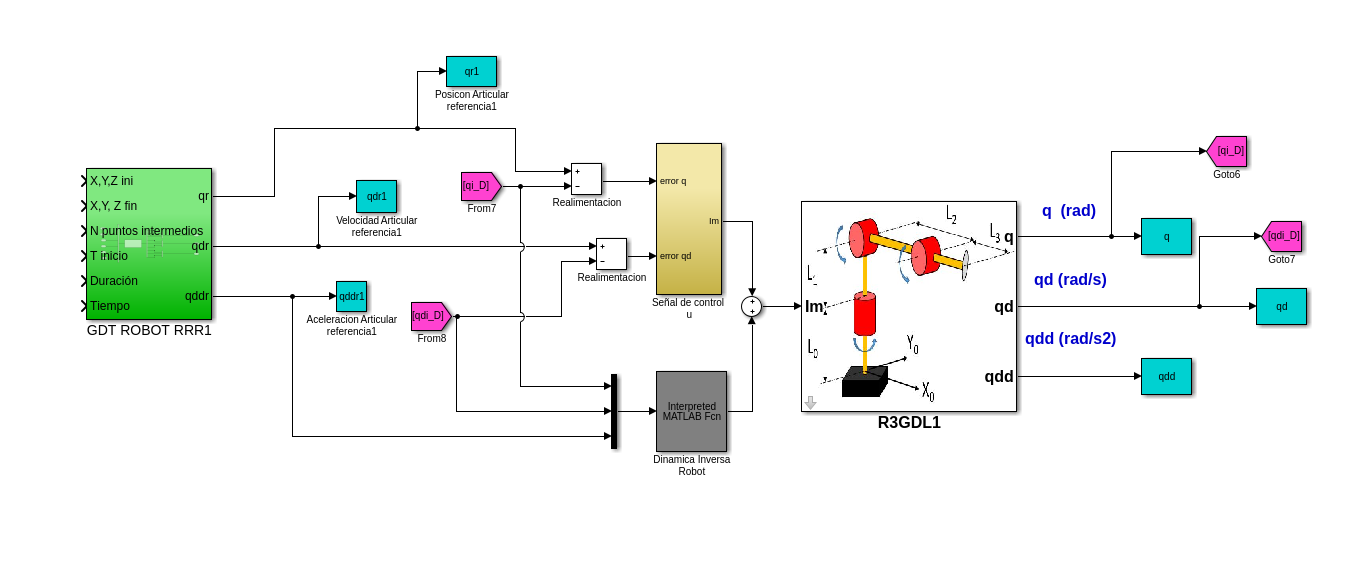
\includegraphics[width=.8\textwidth]{montaje_feedforward}
	\caption{Esquema de un controlador Feed Forward}
\end{figure}

debido a que no se puede medir la aceleración de las variables articulares, cómo se observa, el modelo dinámico inverso del robot se alimentará con los valores de las variables articulares en posición y velocidad y en el caso de la aceleración, se alimentará con la referencia obtenida del generador de trayectorias.

Por lo tanto, a modo de resumen, las funciones de transferencia de las cuales hará que obtener controladores son:
\begin{equation}
	G_{1}(s)=\frac{K_{t1}R_1}{M_{a11}s^{2}} \hspace{2cm} G_{2}(s)=\frac{K_{t2}R_2}{M_{a22}s^{2}} \hspace{2cm} G_{3}(s)=\frac{K_{t3}R_3}{M_{a33}s^{2}}
\end{equation}


	\subsubsection{Controlador PD/PID con par calculado}
	El control mediante par calculado será el último en implementar en éste proyecto. El par calculado se basa en la intención de desacoplar totalmente las interaciones del robot, resultando la dinámica del error cómo un doble integrador, para el cuál habrá que diseñar controladores. \\
	%AÑADIR MAS FANTASIA
	Por tanto, la diferencia de éste controlador frente al resto es que es un controlador dinámico. Además, es un controlador totalmente basado en el modelo, lo que conlleva que si el modelo es malo el control también lo será.
	Si, al igual que antes, se resta al sistema la señal de control que se desea implementar, se obtendrá la dinámica del error:
	\begin{equation}
		\begin{array}{llll}
		  & Im=M_{A}(q)\ddot{q} + C_{A}(q,\dot{q})\dot{q} + G_{A}(q) \\
		- & Im=M_{A}(q)\ddot{q_{ref}+u} + C_{A}(q,\dot{q})\dot{q} + G_{A}(q) \\
		\cline{1-4}
		\vspace{0.2cm}
		  & \tilde{\ddot{q}} = u & &
		\end{array}
	\end{equation}

	Por tanto, las funciones de transferencia a partir de las cuales hay que diseñar los controladores serán:
	\begin{equation}
		G_{1}(s)=\frac{1}{s^{2}} \hspace{2cm} G_{2}(s)=\frac{1}{s^{2}} \hspace{2cm} G_{3}(s)=\frac{1}{s^{2}}
	\end{equation}

	Y, el esquema de control del par calculado se muestra a continuación
		\begin{figure}[h!]
			\centering
			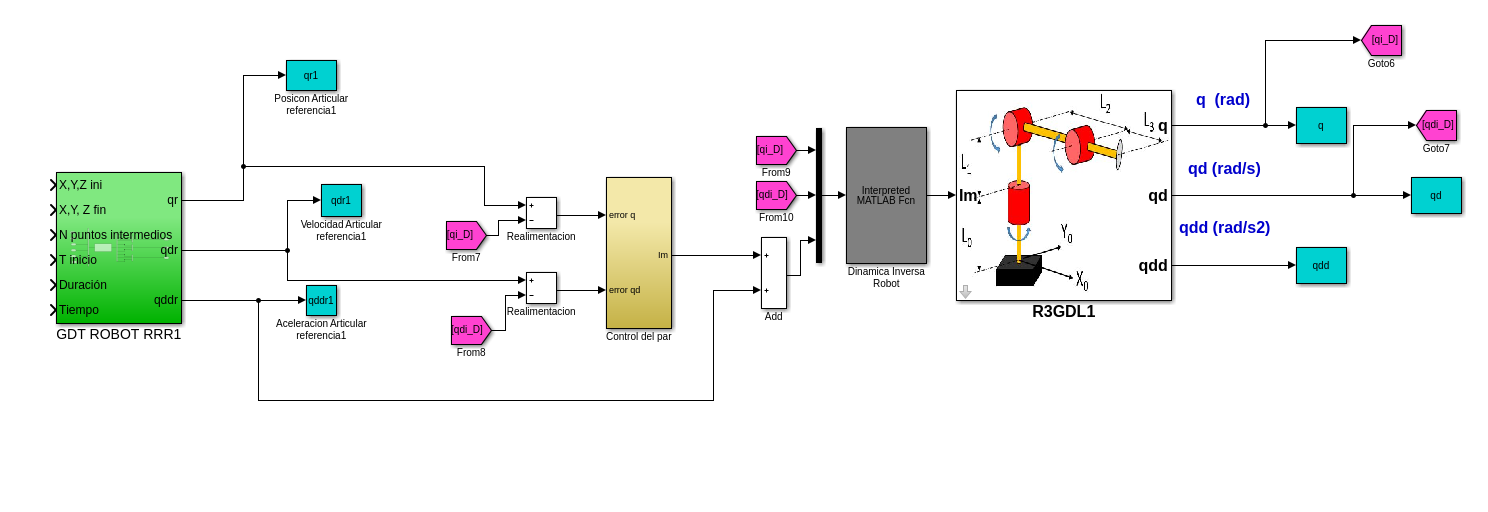
\includegraphics[width=.8\textwidth]{montaje_parcalcul}
			\caption{Esquema de un controlador Par Calculado}
		\end{figure}

























	\subsection{Analisis de controladores}
